\documentclass[conference]{IEEEtran}
\IEEEoverridecommandlockouts
% The preceding line is only needed to identify funding in the first footnote. If that is unneeded, please comment it out.
\usepackage{cite}
\usepackage{amsmath,amssymb,amsfonts}
\usepackage{algorithmic}
\usepackage{graphicx}
\usepackage{textcomp}
\usepackage{xcolor}
\def\BibTeX{{\rm B\kern-.05em{\sc i\kern-.025em b}\kern-.08em
    T\kern-.1667em\lower.7ex\hbox{E}\kern-.125emX}}
\begin{document}

\title{Difficult Text Analysis of Machine Translation Services base on
  Metamorphic Testing in Social Media}

\author{\IEEEauthorblockN{1\textsuperscript{st} Boyang Yan}
\IEEEauthorblockA{\textit{Research Center of Network and Communications} \\
\textit{Peng Cheng Laboratory}\\
Shenzhen, China \\
yanby@pcl.ac.cn}
\and
\IEEEauthorblockN{2\textsuperscript{nd} Given Name Surname}
\IEEEauthorblockA{\textit{dept. name of organization (of Aff.)} \\
\textit{name of organization (of Aff.)}\\
City, Country \\
email address}
\and
\IEEEauthorblockN{3\textsuperscript{rd} Given Name Surname}
\IEEEauthorblockA{\textit{dept. name of organization (of Aff.)} \\
\textit{name of organization (of Aff.)}\\
City, Country \\
email address}
\and
\IEEEauthorblockN{4\textsuperscript{th} Given Name Surname}
\IEEEauthorblockA{\textit{dept. name of organization (of Aff.)} \\
\textit{name of organization (of Aff.)}\\
City, Country \\
email address}
\and
\IEEEauthorblockN{5\textsuperscript{th} Given Name Surname}
\IEEEauthorblockA{\textit{dept. name of organization (of Aff.)} \\
\textit{name of organization (of Aff.)}\\
City, Country \\
email address}
\and
\IEEEauthorblockN{6\textsuperscript{th} Given Name Surname}
\IEEEauthorblockA{\textit{dept. name of organization (of Aff.)} \\
\textit{name of organization (of Aff.)}\\
City, Country \\
email address}
}

\maketitle

\begin{abstract}
  A huge amount of text comments are posted on different topics in Social Media
  every day. These topics are discussed in different languages by different
  language speakers. Most people encounter language and culture barriers when
  engaging in cross-language communication.
  Cross-language machine translation is useful for global integration.
  However, most of people are chosen human translation services.
  The reason is human translation services are accuracy and reliable compare
  with machine translation.
  Most research only focuses on ranking the quantity of machine translation
  services but little research has conducted on difficult translation text
  evaluation.
  This research explores what kind of text is difficult to translate for machine
  translation services base on movie comments data. It is useful for improve the quality
  of machine translation services to fill this research gap.
  This research is based on the Metamorphic Testing method to establish a
  testing model which using machine translation service translate original test
  dataset from one language to another language. After, using sentiment analysis
  tool to analyize original test dataset and translated dataset, the results
  should be same polarization (positive or negative). If the results are
  opposite polarization, that means this sentence is difficult for machine
  translation.
  As a result, people will able to use this testing model finding difficult
  sentences and doing specific optimiztion.
\end{abstract}

\begin{IEEEkeywords}
  Metamorphic Testing, machine translation, sentiment analysis, machine
  translation quantity testing, evaluation of machine translation services difficult
\end{IEEEkeywords}

\section{Introduction}
Machine translation services has been becoming more and more widely used, also
more and more popular. Most people encounter language and cultural barriers
during cross-language communication. There are lots of text and documents on different languages need
to translation every day. It would be impossible to translation the huge amount
of data generated manually. Nowadays, there are lots of machine translation
tools are available in the world, such as Google translation, Bing translation,
Yandex, Baidu translation and Youdao translation and so on. In this research,
only compare and evaluation Google translation, Yandex translation and Baidu
translation difficults. Those three translation tools are typical and the most
widespread to used. Google translation tool come from American, Yandex come from
Russia, and Baidu come from China. Accounting to Pesu said machine translation
tools can product better results on European languages compare with Asian
language \cite{pesu2018monte}. So, Chinese to English translation tool is the main
kind of translation languages to analysis translation difficults in the paper.
Evaluation of machine translation services difficults usually need language
expert, who need well-known both languages, to participate. However, language
expert also involves human emotional judgment. Automatic assessment human
language is naturally difficult because of without a test oracle \cite{zhou2016metamorphic}.
In this paper, achieving a testing modle to automatic assessment
without language expert. Metamorphic testing(MT) is one of property-based
software quality testing method, which alreadly be appoved effective for
addressing the non-oracle problem, such as testing the quality of search engine
and the quality of Unmanned Aerial Vehicle(UAV) flight control application and so on.
Therefore, decideing metamorphic testing to find machine translation services
difficults in non-oracle sitation.
And more specifically, this research raise two questions.
\begin{itemize}
  \item Q1: What is current sitation of the quantity of Chinese to English
    machine translation?
  \item Q2: What is current machine translation difficults between Chinese and English?
\end{itemize}

The rest of paper is organized as three parts. Firstly, domonstration the
quantity of Chinese to English translation services, which are Google
translation, Yandex translation and Baidu translation. This part addresses Q1.
secondly, describtion testing model about finding the difficults of machine
translation.
Thirdly, analyzes the experimental results and discussion. This part will
answer Q2.

\section{Background}
\subsection{Metamorphic Testing}
Metamorphosis Testing(MT) a method for generating test cases, as well as test
results verification. The most importance component is the metamorphic
relation (MR). MR is the target application's necessary properties of function in relation to multiple
inputs and their expected outputs.
In software testing research field, an incapacity to decide, software product
the correct output, is called the oracle problem. This usually means cannot
provide exact correctness reference data. such as, machine translation. Huge and
complexity systems is very common, no
When people want to assess the the accuracy of $\sin$ function. For example, $\sin(2.7)$ is very difficult to
make a correctness judgment from mathematics aspect. If using Metamorphic
Testing method to testing $\sin$ function will reduce computational costs and
more efficient. There is a testing procedures' example for $\sin$ function.
\begin{enumerate}\label{itm:procedures}
\item set a Metamorphic Relation: such as $$\sin(\alpha) = \cos(\frac{\pi}{2} - \alpha)$$
\item $\sin(2.7)$ and $\cos(\frac{\pi}{2} - 2.7)$ should have same output, if the
  outputs are different. We can say, the failure have been detected.
\end{enumerate}
However, when using \ref{itm:procedures}'s testing procedures. someone maybe
ask, $\cos$ function also not reliable, how can use a unreliable function to
test another function's correctness. There have the boundedness. However, both
function have got failures at same time, that is small probability event.

In software testing, an inability to determine if software is behaving
correctly, or producing the correct output, is called the oracle problem [1]. Metamorphic testing (MT) is an approach that can alleviate
the oracle problem [6, 10], MT has been investigated and adopted by
a growing number of researchers and practitioners [7, 16, 20, 21, 28],
successfully uncovering software problems, even in extensively
tested systems [8, 9, 19]. Central to MT is a set of metamorphic
relations (MRs), which are expected relations among the inputs and
outputs of multiple executions of the intended program’s functionality. Instead of examining the behaviour or output for an individual
input, MT checks the SUT against selected MRs, with violations of
an MR indicating the presence of a fault.
An example MR for a database management system is that the
system should return the same results for a query with the search
condition “A and B” and a query with the search condition “B and
A”.
\subsection{Sentiment Analysis}

\section{domonstration the current quantity of Chinese to English translation services}

\subsection{Test Sample}
All of test sample came from Douban, one of biggest social networking service
platforms in China. This social website attracts more than one hundred million
active visitors per month, and has amassed over sixty-five million registered
users. We then employ the Douban public Application Programming Interfaces
(APIs) to access Chinses-written comments. A typical data structure of harvested
comment is shown as a tuple: [Rating, Raw comments]. Totally, comments have got
46180 in the corpus. User rating total have 5 groups, which are 10, 20, 30, 40
and 50, from negative to positive.
The test sample distribution diagram on below.
\centerline{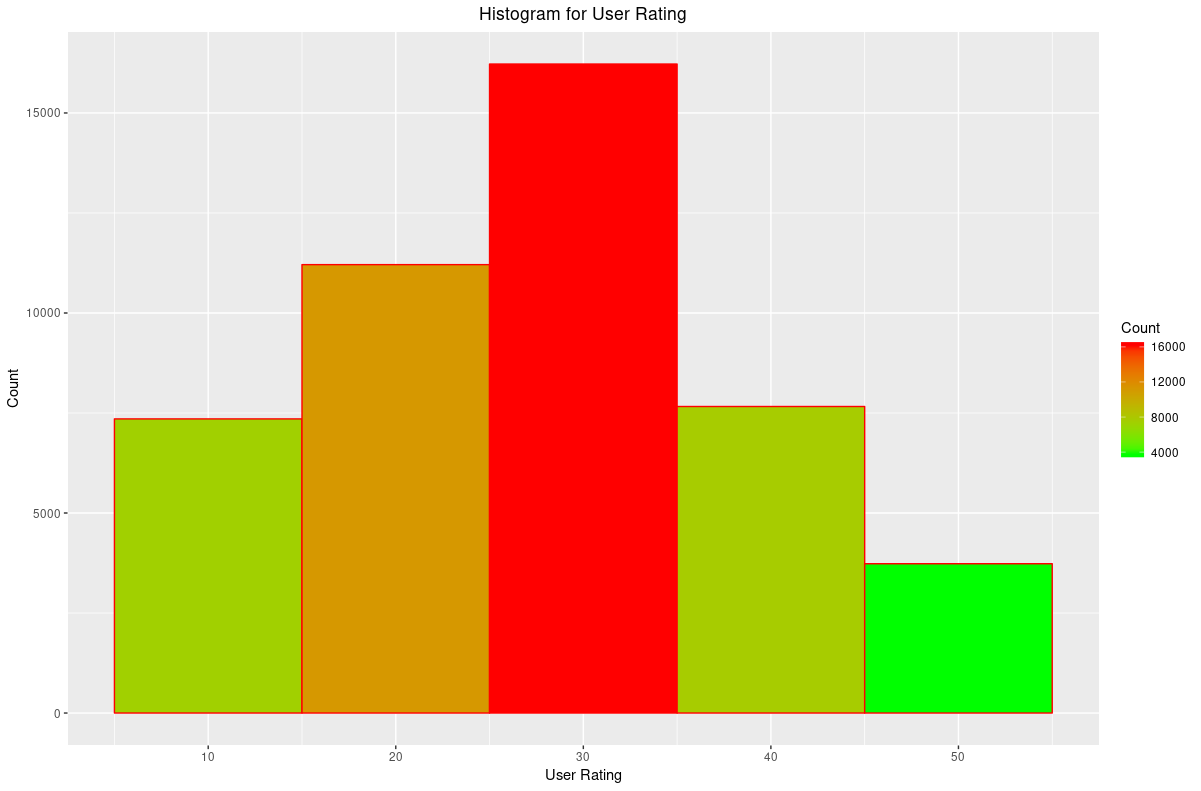
\includegraphics[width=0.3\paperwidth]{./img/ratingHis.png}}
As you can see, the majority of comments allocate on rating 30. In addition,
there have got more negative comments compare with positive comments.

\subsection{Testing procedures}
\begin{enumerate}
  \item using three of machine translation services to translate Chinese
    original movie comments to English translated movie comments.
    $$P_{(Origin Data)} \rightarrow P^{\prime}_{(Google Translation)}$$
    $$P_{(Origin Data)} \rightarrow P^{\prime}_{(Yandex Translation)}$$
    $$P_{(Origin Data)} \rightarrow P^{\prime}_{(Baidu Translation)}$$
  \item Using Google sentiment analysis tool to analysis $P_{(Origin Data)}$,
    $P^{\prime}_{(Google Translation)}$, $ P^{\prime}_{(Yandex Translation)}$ and $
    P^{\prime}_{(Baidu Translation)}$. Google sentiment analysis APIs will get 2
    values, which are Score and Manitude. The range of Score is between -1 and
    1. If Score more close to 1 means this movie comment more positive, as well
    as, if Score more close to -1 means this movie comment more negative.
  \item Using user rating values (10, 20, 30, 40 or 50) to check Google
    Sentiment Analysis(SA) results $P_{(Origin Data)} $ is True or False. For example, user rating = 10 and Google Chinese SA score between -1
    and -0.6 (mean True) user ranking = 10 and Google Chinese SA score bigger
    than -0.6 (mean False). The decideing True table on below. Else Not in True
    table all False.\\
    \begin{center}
      \begin{tabular}{|c|c|c|c|}
        \hline
        user rating & Google SA score & True/False \\
        \hline\hline
        10 & $[ \, -1, -0.4 ] \,$ & True \\
        \hline
        20 & $[ \, -0.8, 0 ] \,$ & True \\
        \hline
        30 & $[ \, -0.4, 0.4 ] \,$ & True \\
        \hline
        40 & $[ \, 0, 0.8 ] \,$ & True \\
        \hline
        50 & $[ \, 0.4, 1 ] \,$ & True \\
        \hline
      \end{tabular}
    \end{center}
  \item Using those True or False values as vector combining with Google English
    SA scores (based on $P^{\prime}_{(Google Translation)}$), Google English SA
    scores (based on $ P^{\prime}_{(Yandex Translation)}$) and Google English SA
    scores (based on $P^{\prime}_{(Baidu Translation)}$) draw 3 Receiver operating
    characteristic (ROC) graphics and 3 Precision-recall curves (PRC) graphics.

    ROC curve is often used in evaluation the clinical performance of a
    biochemical test. The ROC curve is based on a series of different binary
    classifier with the true positive rate (sensitivity) as the Y-axis and the
    false positive rate (1-specificity) as the X-axis \cite{ROC}. The traditional
    evaluation must be divided into two categories, and then statistical
    analysis is performed. The ROC curve is different from the traditional
    evaluation method. Instead, an intermediate state is allowed. The test
    results can be divided into multiple ordered classifications then
    statistically analyzed. However, visual interpretation and comparisons of
    ROC curves based on imbalanced data sets can be misleading. An alternative
    to a ROC curve is a precision-recall curve (PRC). PRC might be a better
    choice for imbalanced datasets \cite{davis2006relationship}.
    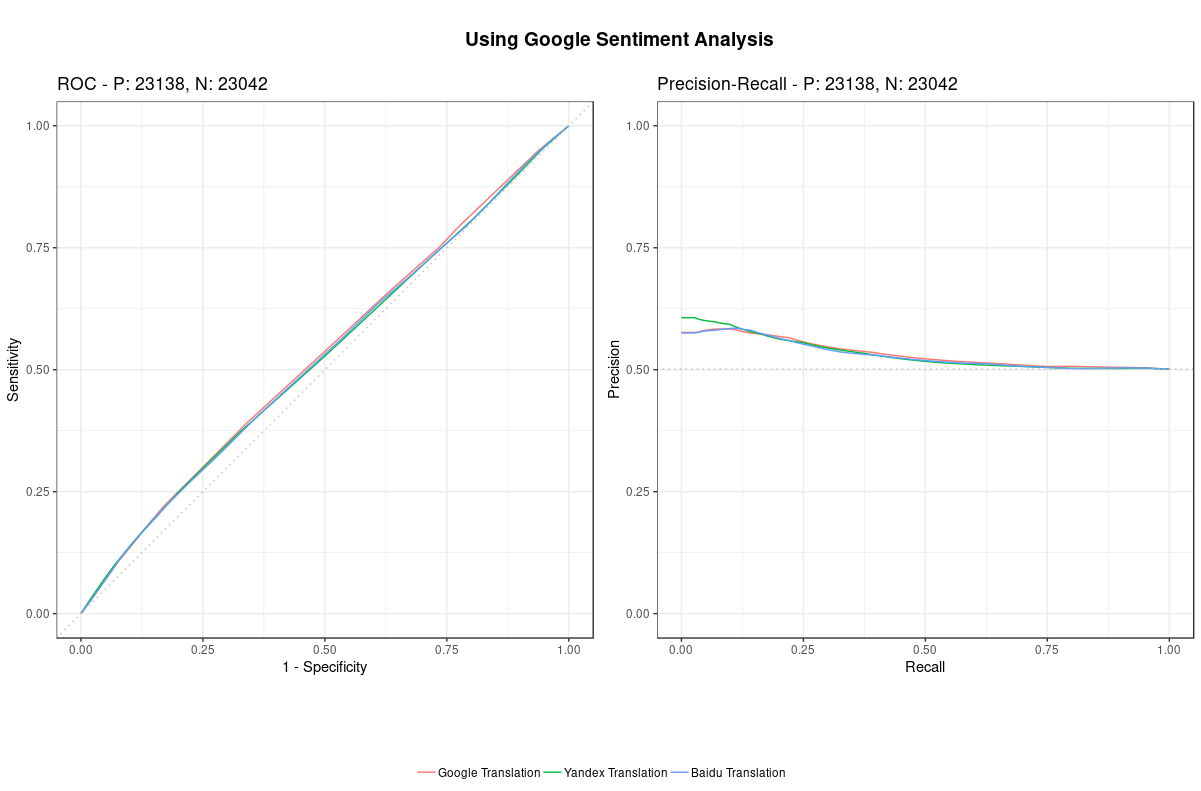
\includegraphics[width=0.35\paperwidth]{./img/ROCandPRC.png}
    This graphic show those three of machine translation tools all achieve poor
    translation results.
  \item Calculate Area Under The Curve (AUC) values for ROC and PRC.
    \begin{table}[h]
      \caption {Google Translation}
    \begin{center}
      \begin{tabular}{|c|c|}
        \hline
        Curve Types & AUCs \\
        \hline\hline
        ROC & 0.5307797 \\
        \hline
        PRC & 0.5328503 \\
        \hline
      \end{tabular}
    \end{center}
  \end{table}\\
   \begin{table}[h]
     \caption {Yandex Translation}
     \begin{center}
       \begin{tabular}{|c|c|}
         \hline
         Curve Types & AUCs \\
         \hline\hline
         ROC & 0.5251734 \\
         \hline
         PRC & 0.5322736 \\
         \hline
       \end{tabular}
     \end{center}
   \end{table}\\
  \begin{table}[h]
    \caption {Baidu Translation}
    \begin{center}
      \begin{tabular}{|c|c|}
        \hline
        Curve Types & AUCs \\
        \hline\hline
        ROC & 0.5258386 \\
        \hline
        PRC & 0.5302736 \\
        \hline
      \end{tabular}
    \end{center}
  \end{table}\\
  The AUC is between 1.0 and 0.5. The better diagnostic effect will be close to 1.
  \begin{itemize}
  \item AUC has lower accuracy from 0.5 to 0.7
  \item AUC has a certain accuracy from 0.7 to 0.9
  \item AUC has higher accuracy at above 0.9
  \end{itemize}
  When AUC=0.5, it means that the diagnostic method is completely ineffective
  and has no diagnostic value \cite{baiduROC}.
  \begin{itemize}
  \item For ROC AUCS: It shows \textbf{Google Translation tool} better than
    \textbf{Baidu Translation tool} better than \textbf{Yandex Translation tool}
    \item For PRC AUCS: It shows \textbf{Googl Translation tool} better than
      \textbf{Yandex Translation tool} better than \textbf{Baidu Translation
        tool}
  \end{itemize}

\begin{itemize}
\item The number of true value: 23042
\item The number of false value: 23138
\end{itemize}

\end{enumerate}
Alought the dataset is looks balanced, ROC diagram can be trusted. The ranking
of machine translation services' quantity are NOT reliable. The reason is three of translation services
have lower accuracy. In another word, working not properly correct.

\subsection{finding the difficults of machine translation}
\subsection{Testing procedures}
\begin{enumerate}
    \item using three of machine translation services to translate Chinese
    original movie comments to English translated movie comments.
    $$P_{(Origin Data)} \rightarrow P^{\prime}_{(Google Translation)}$$
    $$P_{(Origin Data)} \rightarrow P^{\prime}_{(Yandex Translation)}$$
    $$P_{(Origin Data)} \rightarrow P^{\prime}_{(Baidu Translation)}$$
  \item Using Google sentiment analysis tool to analysis $P_{(Origin Data)}$,
    $P^{\prime}_{(Google Translation)}$, $ P^{\prime}_{(Yandex Translation)}$ and $
    P^{\prime}_{(Baidu Translation)}$. The result are $SA_{(Origin Data)}$,
    $SA^{\prime}_{(Google Translation)}$, $ SA^{\prime}_{(Yandex Translation)}$ and $
    SA^{\prime}_{(Baidu Translation)}$
  \item This three of relations should NOT be opposite attitude
\begin{itemize}
  \item R1: $$SA_{(Origin Data)} \longleftrightarrow SA^{\prime}_{(Google Translation)}$$
  \item R2: $$SA_{(Origin Data)} \longleftrightarrow SA^{\prime}_{(Yandex Translation)}$$
  \item R3: $$SA_{(Origin Data)} \longleftrightarrow SA^{\prime}_{(Baidu Translation)}$$
\end{itemize}

\end{enumerate}

\subsection{Analysis}
R1, R2 and R3 have got failures decideing by one side greater than 0.7 and
another side smaller than -0.7. In this paper, using veen diagram for show
failures distribution.
  \begin{table}[h]
    \caption {Translation Failures Distribution}
    \begin{center}
      \begin{tabular}{|c|c|}
        \hline
        Types & Number Of Failures \\
        \hline\hline
        google Translation & 137\\
        \hline
        Yandex & 129 \\
        \hline
        Baidu & 134 \\
        \hline
        $Google \cap Baidu$ & 38 \\
        \hline
        $Google \cap Yandex$ & 46 \\
        \hline
        $Yandex \cap Baidu$ & 37 \\
        \hline
        $Yandex \cap Baidu \cap Google$ & 17 \\
        \hline
      \end{tabular}
    \end{center}
  \end{table}\\

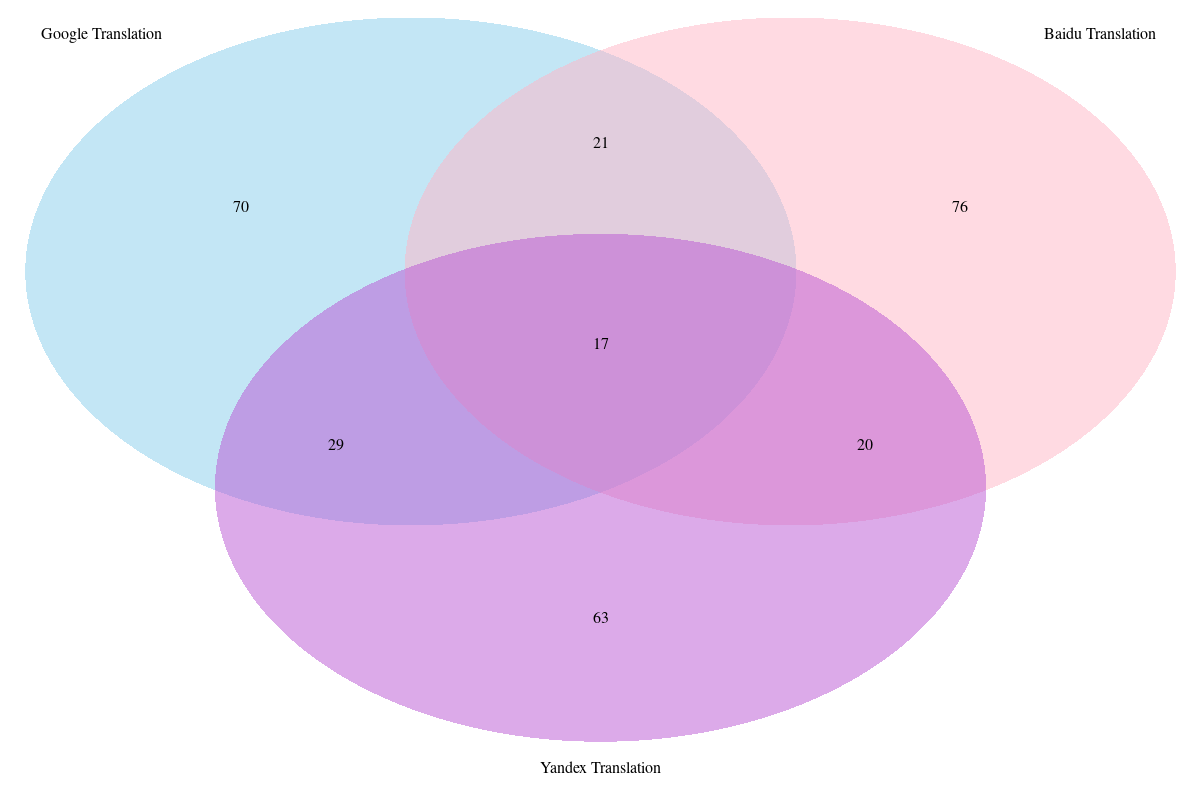
\includegraphics[width=0.35\paperwidth]{./img/veen.png}


\bibliographystyle{IEEEtran}
\bibliography{library}
\end{document}
